% Options for packages loaded elsewhere
\PassOptionsToPackage{unicode}{hyperref}
\PassOptionsToPackage{hyphens}{url}
\PassOptionsToPackage{dvipsnames,svgnames,x11names}{xcolor}
%
\documentclass[
  letterpaper,
  DIV=11,
  numbers=noendperiod]{scrartcl}

\usepackage{amsmath,amssymb}
\usepackage{lmodern}
\usepackage{iftex}
\ifPDFTeX
  \usepackage[T1]{fontenc}
  \usepackage[utf8]{inputenc}
  \usepackage{textcomp} % provide euro and other symbols
\else % if luatex or xetex
  \usepackage{unicode-math}
  \defaultfontfeatures{Scale=MatchLowercase}
  \defaultfontfeatures[\rmfamily]{Ligatures=TeX,Scale=1}
\fi
% Use upquote if available, for straight quotes in verbatim environments
\IfFileExists{upquote.sty}{\usepackage{upquote}}{}
\IfFileExists{microtype.sty}{% use microtype if available
  \usepackage[]{microtype}
  \UseMicrotypeSet[protrusion]{basicmath} % disable protrusion for tt fonts
}{}
\makeatletter
\@ifundefined{KOMAClassName}{% if non-KOMA class
  \IfFileExists{parskip.sty}{%
    \usepackage{parskip}
  }{% else
    \setlength{\parindent}{0pt}
    \setlength{\parskip}{6pt plus 2pt minus 1pt}}
}{% if KOMA class
  \KOMAoptions{parskip=half}}
\makeatother
\usepackage{xcolor}
\setlength{\emergencystretch}{3em} % prevent overfull lines
\setcounter{secnumdepth}{-\maxdimen} % remove section numbering
% Make \paragraph and \subparagraph free-standing
\ifx\paragraph\undefined\else
  \let\oldparagraph\paragraph
  \renewcommand{\paragraph}[1]{\oldparagraph{#1}\mbox{}}
\fi
\ifx\subparagraph\undefined\else
  \let\oldsubparagraph\subparagraph
  \renewcommand{\subparagraph}[1]{\oldsubparagraph{#1}\mbox{}}
\fi


\providecommand{\tightlist}{%
  \setlength{\itemsep}{0pt}\setlength{\parskip}{0pt}}\usepackage{longtable,booktabs,array}
\usepackage{calc} % for calculating minipage widths
% Correct order of tables after \paragraph or \subparagraph
\usepackage{etoolbox}
\makeatletter
\patchcmd\longtable{\par}{\if@noskipsec\mbox{}\fi\par}{}{}
\makeatother
% Allow footnotes in longtable head/foot
\IfFileExists{footnotehyper.sty}{\usepackage{footnotehyper}}{\usepackage{footnote}}
\makesavenoteenv{longtable}
\usepackage{graphicx}
\makeatletter
\def\maxwidth{\ifdim\Gin@nat@width>\linewidth\linewidth\else\Gin@nat@width\fi}
\def\maxheight{\ifdim\Gin@nat@height>\textheight\textheight\else\Gin@nat@height\fi}
\makeatother
% Scale images if necessary, so that they will not overflow the page
% margins by default, and it is still possible to overwrite the defaults
% using explicit options in \includegraphics[width, height, ...]{}
\setkeys{Gin}{width=\maxwidth,height=\maxheight,keepaspectratio}
% Set default figure placement to htbp
\makeatletter
\def\fps@figure{htbp}
\makeatother

\KOMAoption{captions}{tableheading}
\makeatletter
\makeatother
\makeatletter
\makeatother
\makeatletter
\@ifpackageloaded{caption}{}{\usepackage{caption}}
\AtBeginDocument{%
\ifdefined\contentsname
  \renewcommand*\contentsname{Table of contents}
\else
  \newcommand\contentsname{Table of contents}
\fi
\ifdefined\listfigurename
  \renewcommand*\listfigurename{List of Figures}
\else
  \newcommand\listfigurename{List of Figures}
\fi
\ifdefined\listtablename
  \renewcommand*\listtablename{List of Tables}
\else
  \newcommand\listtablename{List of Tables}
\fi
\ifdefined\figurename
  \renewcommand*\figurename{Figure}
\else
  \newcommand\figurename{Figure}
\fi
\ifdefined\tablename
  \renewcommand*\tablename{Table}
\else
  \newcommand\tablename{Table}
\fi
}
\@ifpackageloaded{float}{}{\usepackage{float}}
\floatstyle{ruled}
\@ifundefined{c@chapter}{\newfloat{codelisting}{h}{lop}}{\newfloat{codelisting}{h}{lop}[chapter]}
\floatname{codelisting}{Listing}
\newcommand*\listoflistings{\listof{codelisting}{List of Listings}}
\makeatother
\makeatletter
\@ifpackageloaded{caption}{}{\usepackage{caption}}
\@ifpackageloaded{subcaption}{}{\usepackage{subcaption}}
\makeatother
\makeatletter
\@ifpackageloaded{tcolorbox}{}{\usepackage[many]{tcolorbox}}
\makeatother
\makeatletter
\@ifundefined{shadecolor}{\definecolor{shadecolor}{rgb}{.97, .97, .97}}
\makeatother
\makeatletter
\makeatother
\ifLuaTeX
  \usepackage{selnolig}  % disable illegal ligatures
\fi
\IfFileExists{bookmark.sty}{\usepackage{bookmark}}{\usepackage{hyperref}}
\IfFileExists{xurl.sty}{\usepackage{xurl}}{} % add URL line breaks if available
\urlstyle{same} % disable monospaced font for URLs
\hypersetup{
  pdftitle={Tensed Tendons},
  pdfauthor={Eric Hartmann},
  pdfkeywords={template, demo},
  colorlinks=true,
  linkcolor={blue},
  filecolor={Maroon},
  citecolor={Blue},
  urlcolor={Blue},
  pdfcreator={LaTeX via pandoc}}

\title{Tensed Tendons}
\usepackage{etoolbox}
\makeatletter
\providecommand{\subtitle}[1]{% add subtitle to \maketitle
  \apptocmd{\@title}{\par {\large #1 \par}}{}{}
}
\makeatother
\subtitle{Looking at mechanoradicals in atomic detail}
\author{Eric Hartmann}
\date{7/30/22}

\begin{document}
\maketitle
\ifdefined\Shaded\renewenvironment{Shaded}{\begin{tcolorbox}[enhanced, interior hidden, borderline west={3pt}{0pt}{shadecolor}, breakable, sharp corners, frame hidden, boxrule=0pt]}{\end{tcolorbox}}\fi

\hypertarget{section}{%
\section{}\label{section}}

\hypertarget{are-mechanoradicals-relevant-in-biology}{%
\section{Are mechanoradicals relevant in
biology?}\label{are-mechanoradicals-relevant-in-biology}}

\hypertarget{molecular-dynamics-md-simulations-serve-as-a-computational-microscope}{%
\subsection{Molecular dynamics (MD) simulations serve as a computational
microscope}\label{molecular-dynamics-md-simulations-serve-as-a-computational-microscope}}

\begin{figure}

{\centering 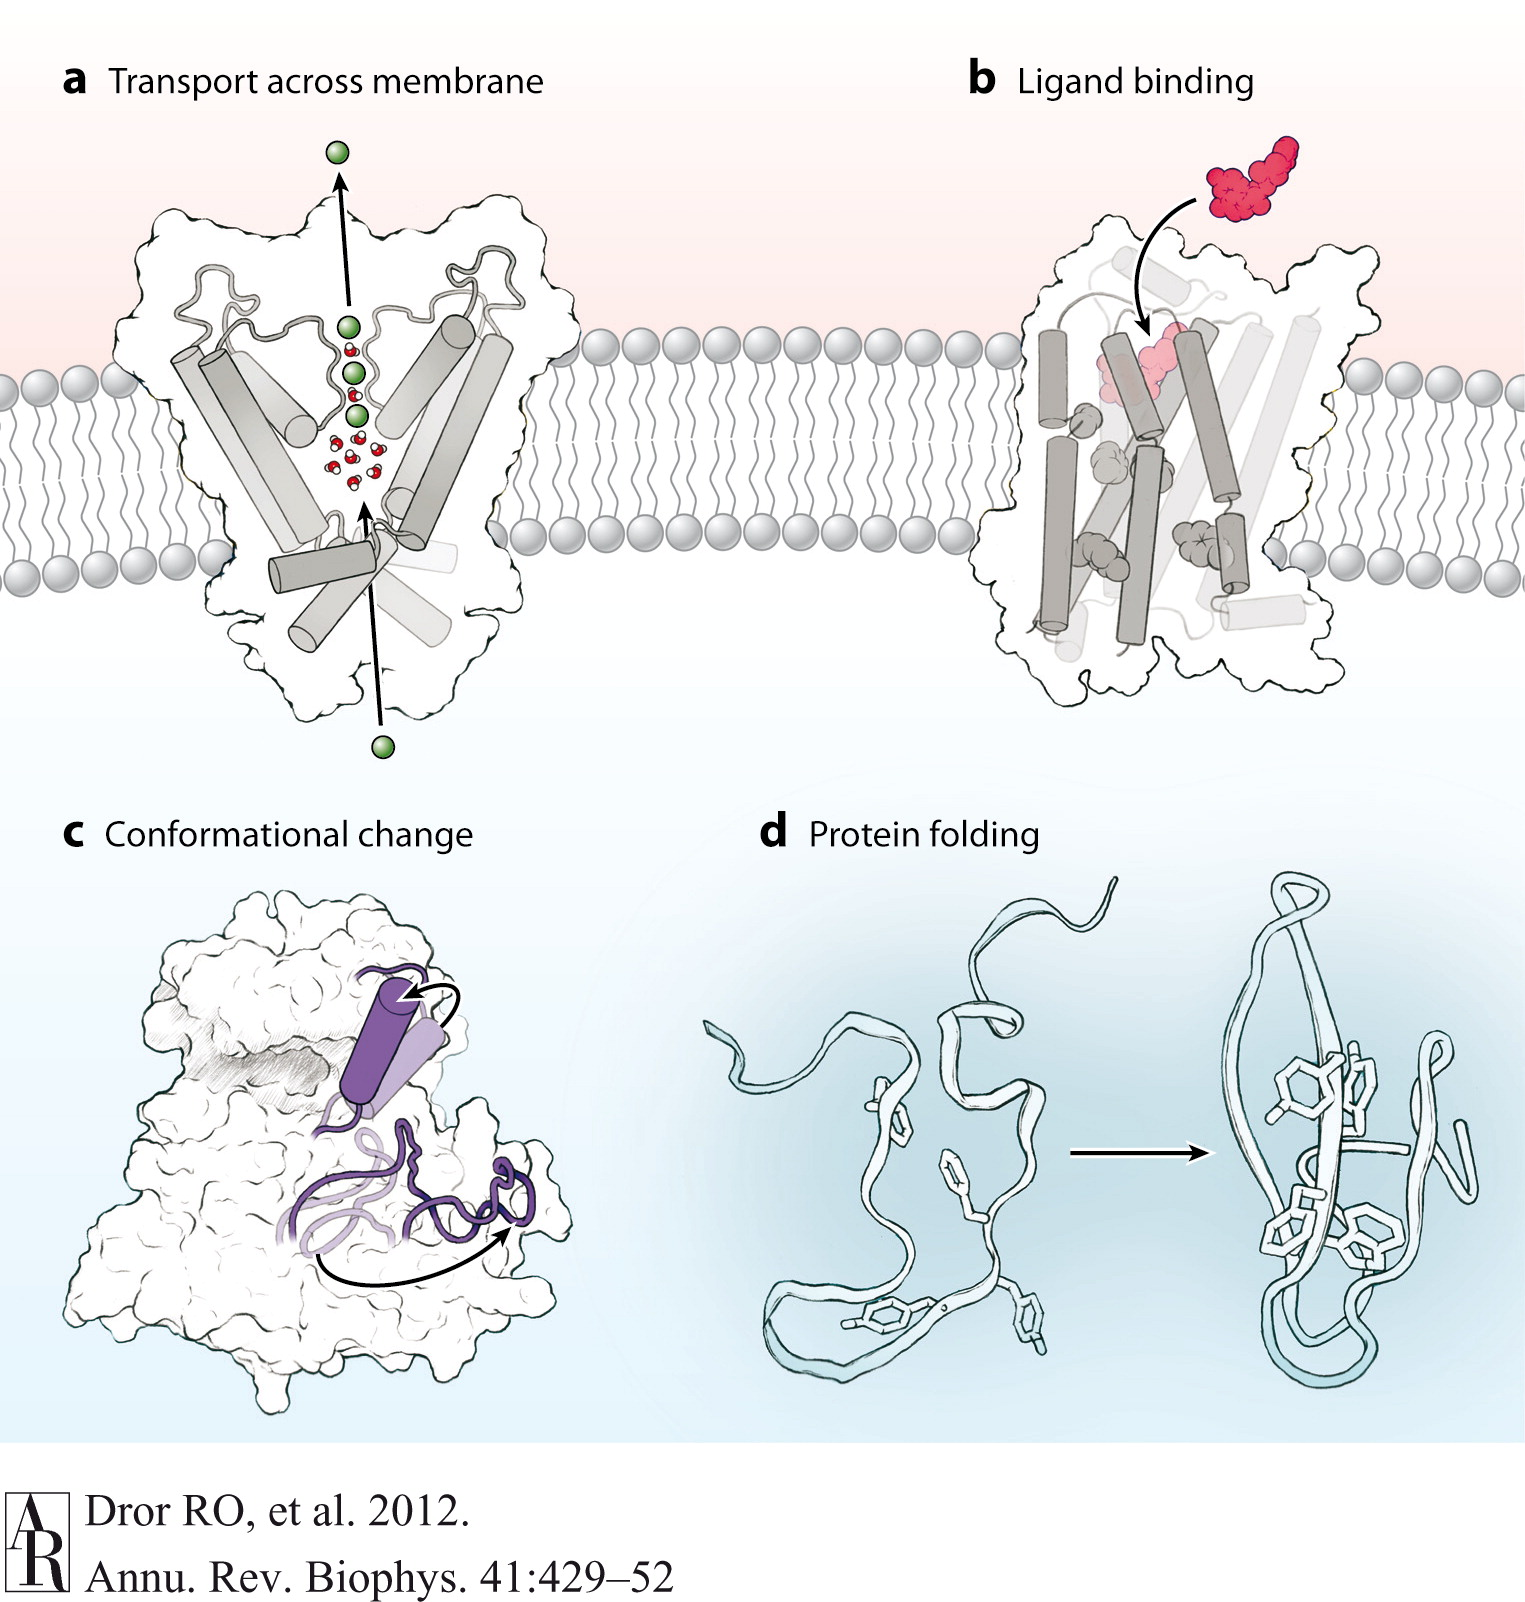
\includegraphics{www/Comp_microscope.jpeg}

}

\end{figure}

\hypertarget{dynamics-of-molecules-are-simulated-by-solving-newtons-equations-of-motion}{%
\subsection{Dynamics of molecules are simulated by solving Newton's
equations of
motion}\label{dynamics-of-molecules-are-simulated-by-solving-newtons-equations-of-motion}}

\[ F_i = \frac{\delta V}{\delta r_i} \qquad \qquad \qquad F_i = m_i * a_i  \qquad \qquad \qquad   \Delta v_i = \frac{\Delta t}{m_i} * F_i(t)
\]

\hypertarget{md-is-based-on-quantum-mechanics}{%
\subsection{MD is based on quantum
mechanics}\label{md-is-based-on-quantum-mechanics}}

\begin{figure}

{\centering 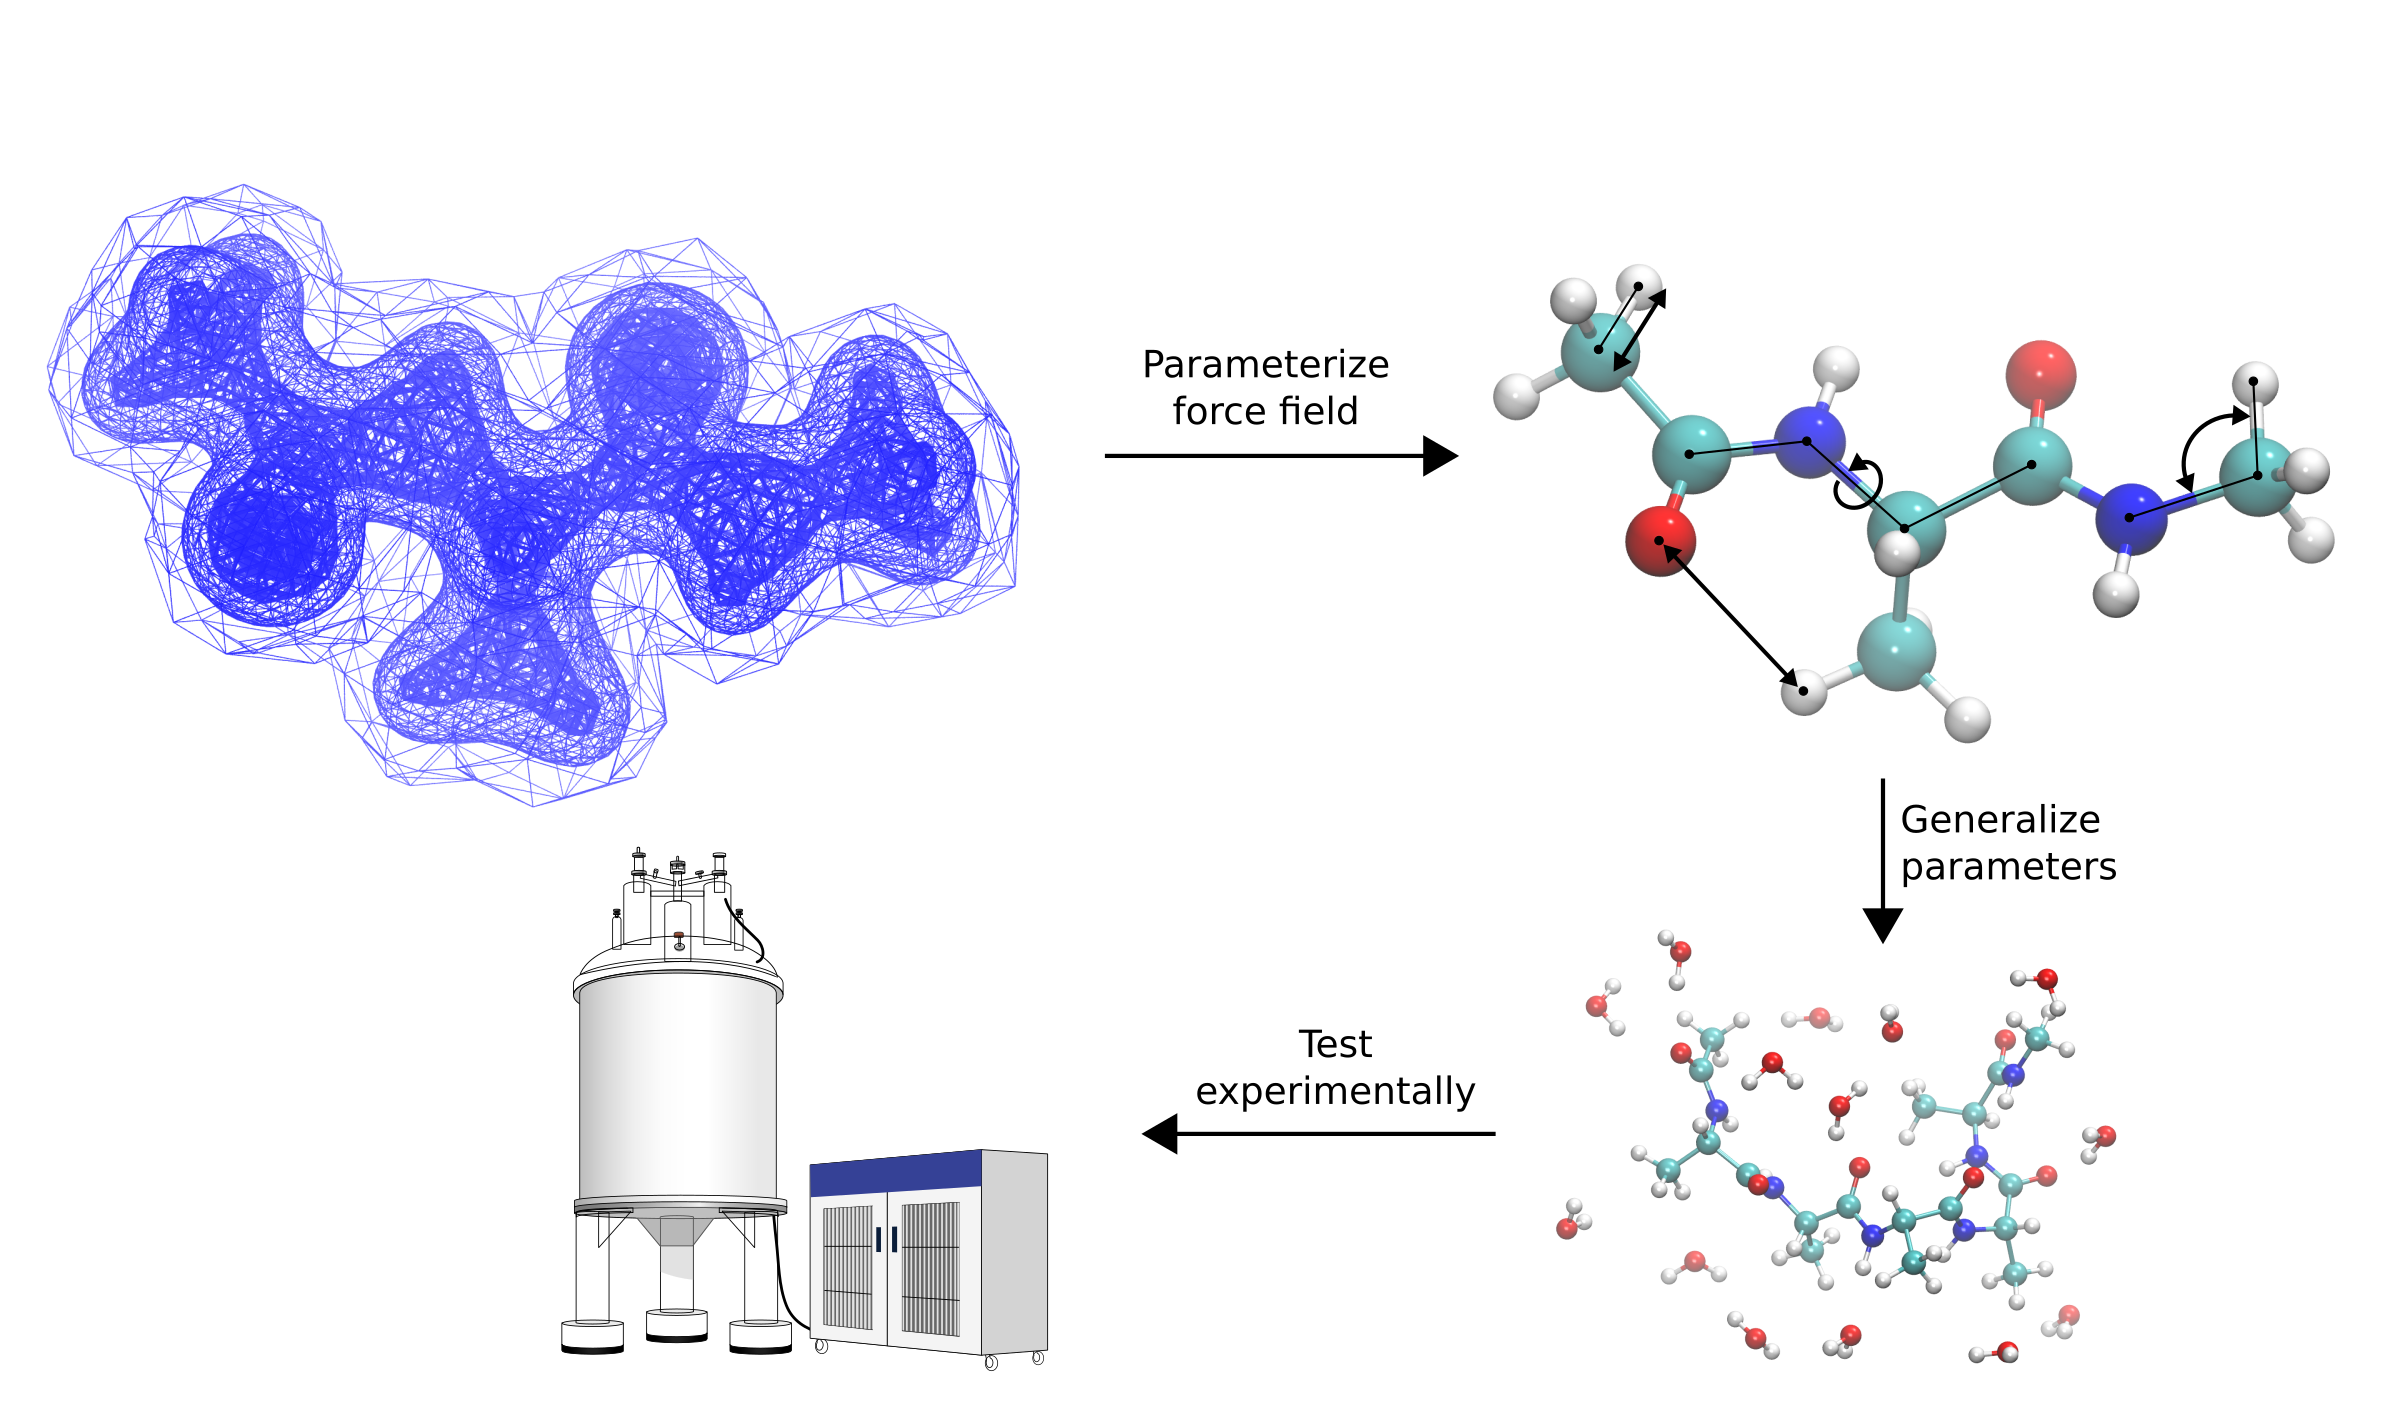
\includegraphics{www/Parameterization_compr.png}

}

\end{figure}

NMR icon from bioicons by simonduerr

\hypertarget{bonds-neither-form-nor-break-in-classical-md-simulations}{%
\subsection{Bonds neither form nor break in classical MD
simulations}\label{bonds-neither-form-nor-break-in-classical-md-simulations}}

\begin{figure}

{\centering 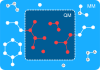
\includegraphics{www/qmmm.svg}

}

\end{figure}

from bioicons by simonduerr

\hypertarget{mdmc-is-a-cheap-reactive-method}{%
\subsection{MD/MC is a cheap reactive
method}\label{mdmc-is-a-cheap-reactive-method}}

\begin{figure}

{\centering 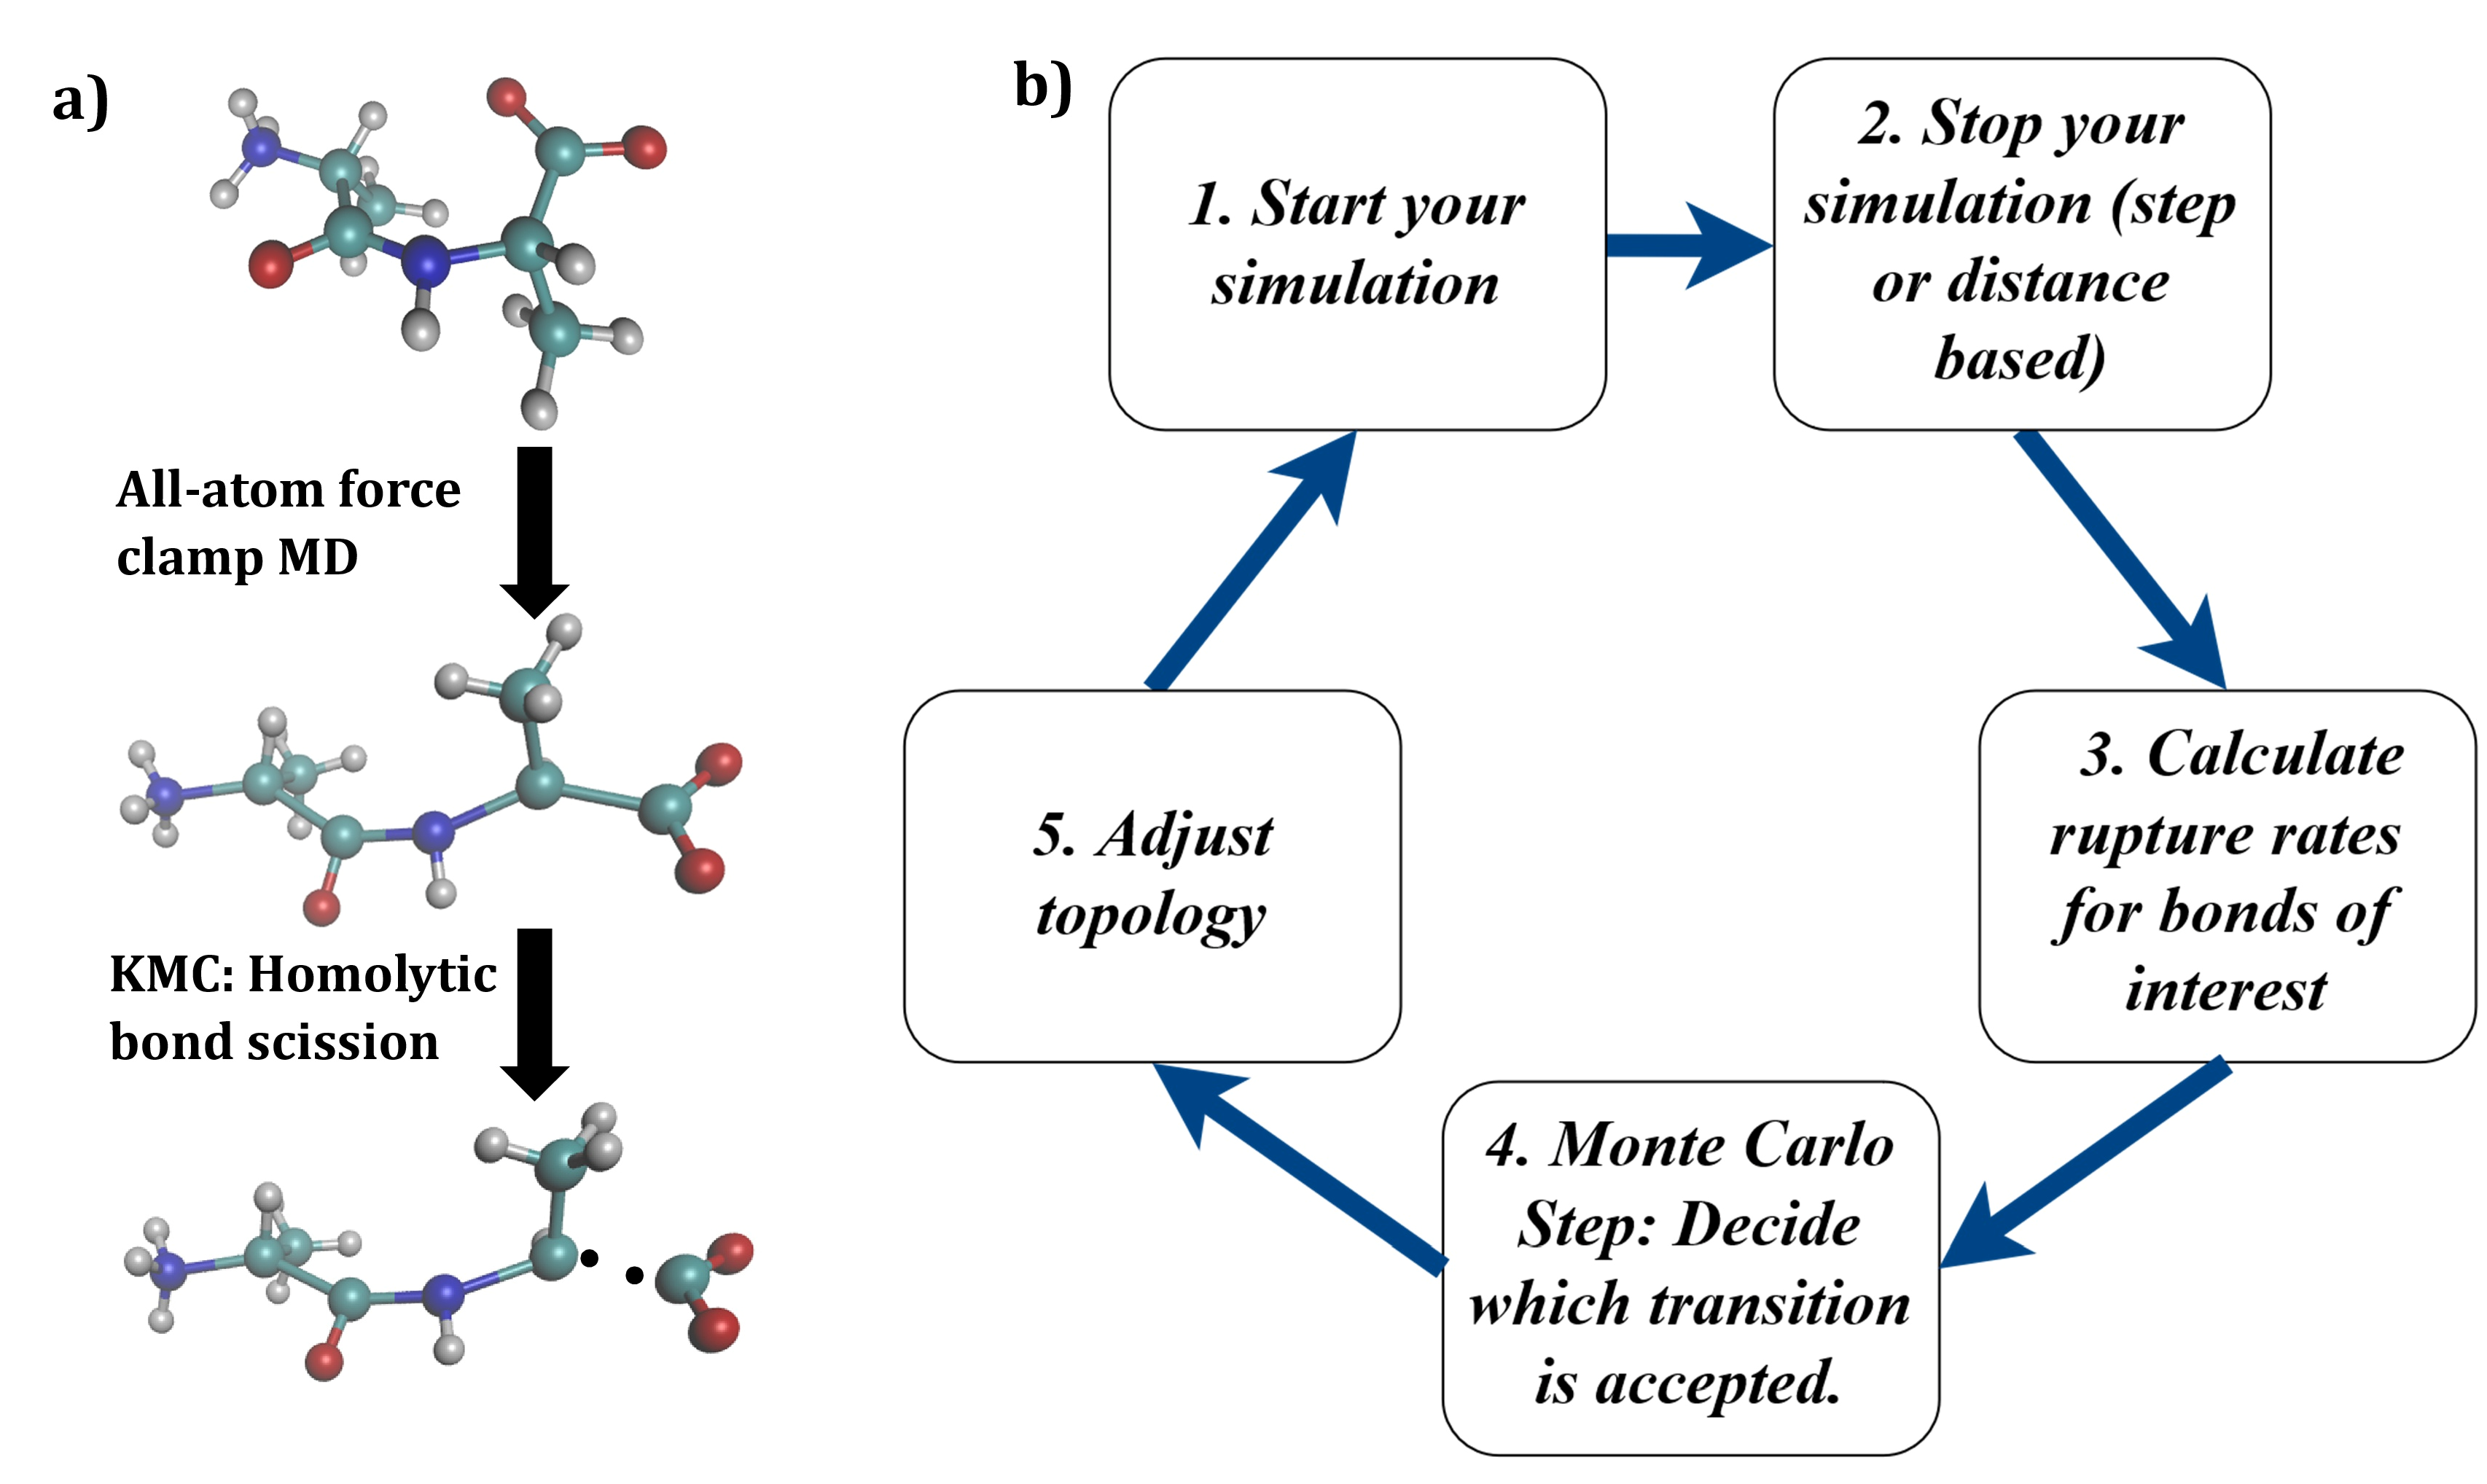
\includegraphics{www/KIMMDY_cycle.png}

}

\end{figure}

Rennekamp et al.~Hybrid Kinetic Monte Carlo/Molecular Dynamics
Simulations of Bond Scissions in Proteins. J. Chem. Theory Comput.
(2020)

\hypertarget{finding-radicals-in-collagen}{%
\section{Finding radicals in
collagen}\label{finding-radicals-in-collagen}}

\hypertarget{stressed-collagen-shows-a-dopa-radical-signal-in-epr}{%
\subsection{Stressed collagen shows a DOPA radical signal in
EPR}\label{stressed-collagen-shows-a-dopa-radical-signal-in-epr}}

\begin{figure}

{\centering 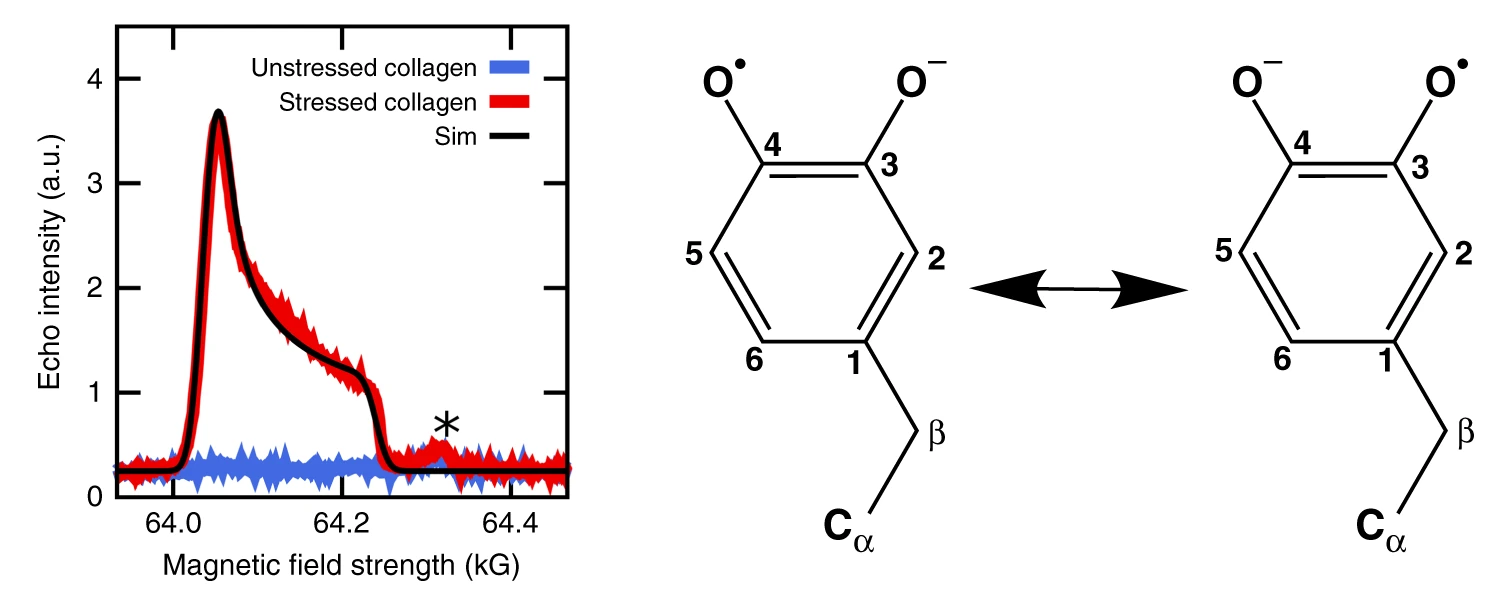
\includegraphics{www/DOPA_EPR.png}

}

\end{figure}

Zapp et al.~Mechanoradicals in tensed tendon collagen as a source of
oxidative stress. Nat Commun (2020).

\hypertarget{dopa-precursors-are-found-near-crosslinks}{%
\subsection{DOPA precursors are found near
crosslinks}\label{dopa-precursors-are-found-near-crosslinks}}

\begin{figure}

{\centering 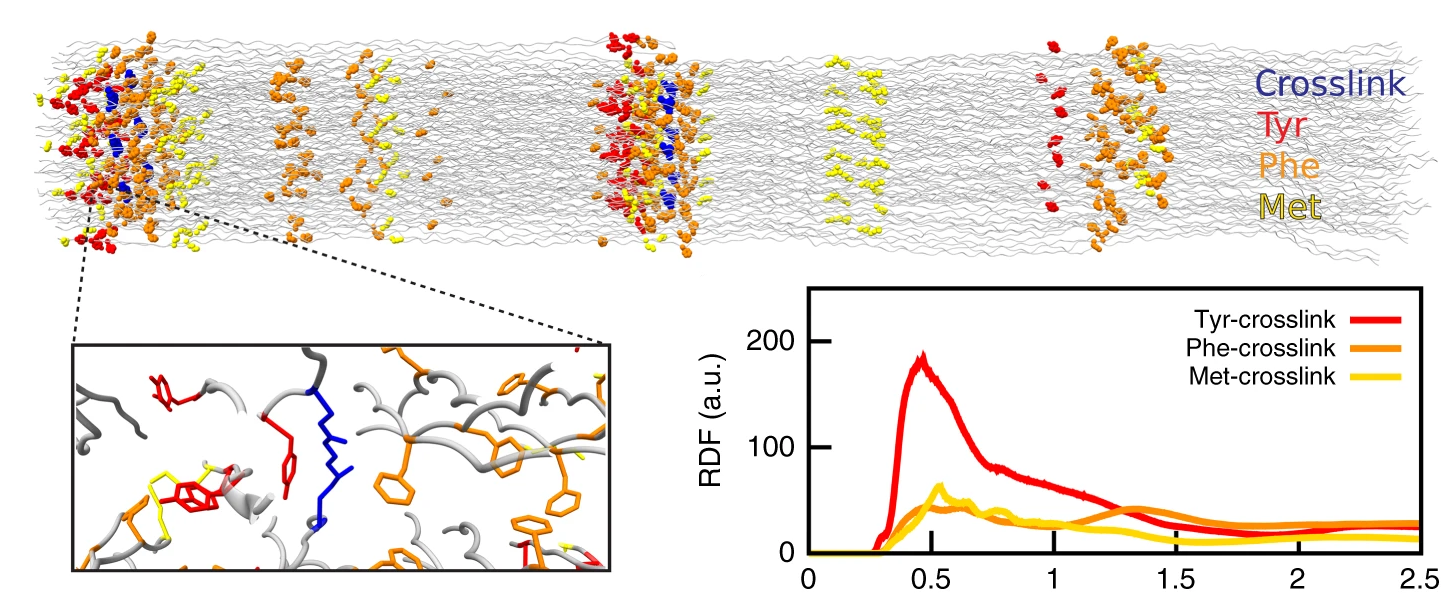
\includegraphics{www/DOPA_Modelling.png}

}

\end{figure}

Zapp et al.~Mechanoradicals in tensed tendon collagen as a source of
oxidative stress. Nat Commun (2020).

\hypertarget{pulling-simulations-suggest-breaks-at-crosslinks}{%
\subsection{Pulling simulations suggest breaks at
crosslinks}\label{pulling-simulations-suggest-breaks-at-crosslinks}}

\begin{figure}

{\centering 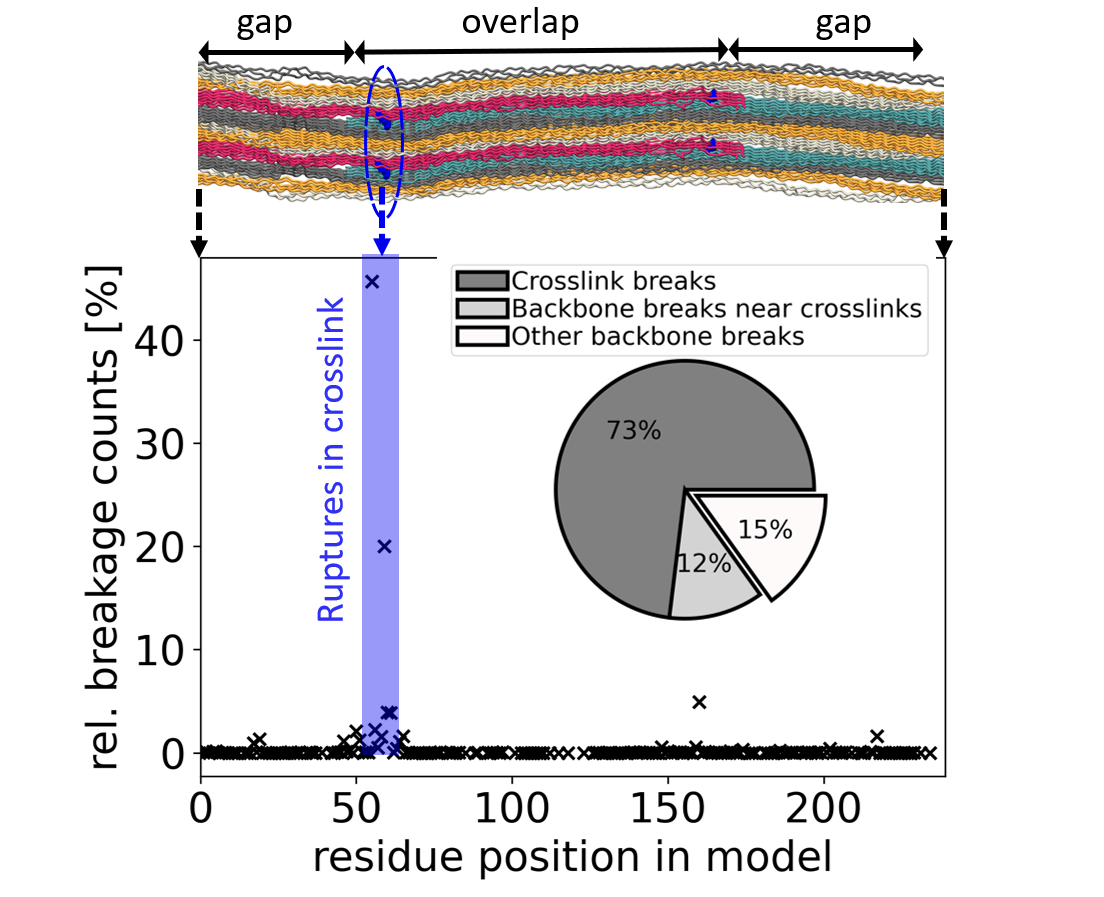
\includegraphics{www/WhereBreak.png}

}

\end{figure}

from Benedikt Rennekamp and Christoph Karfusehr, MBM group

\hypertarget{ms-experiments-confirm-dopa-near-crosslinks}{%
\subsection{MS experiments confirm DOPA near
crosslinks}\label{ms-experiments-confirm-dopa-near-crosslinks}}

\begin{figure}

{\centering 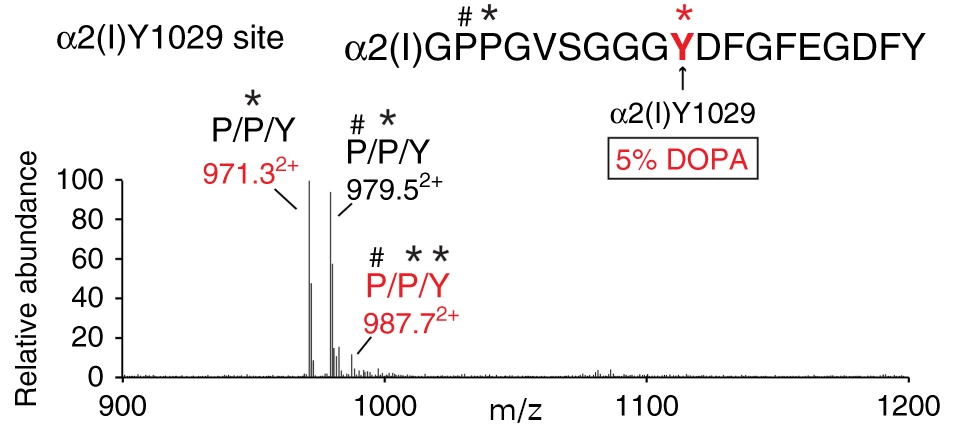
\includegraphics{www/DOPA_MS.png}

}

\end{figure}

Zapp et al.~Mechanoradicals in tensed tendon collagen as a source of
oxidative stress. Nat Commun (2020).

\hypertarget{the-radical-transfer-to-dopa-is-a-missing-link}{%
\subsection{The radical transfer to DOPA is a missing
link}\label{the-radical-transfer-to-dopa-is-a-missing-link}}

\begin{figure}

{\centering 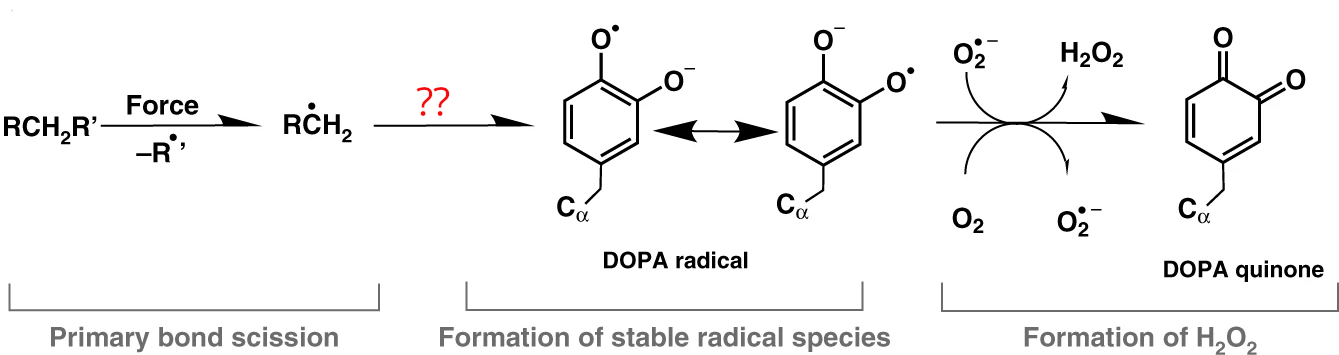
\includegraphics{www/Collagen_mechanism.png}

}

\end{figure}

\hypertarget{reactive-md-shows-radical-migration-pathways}{%
\subsection{Reactive MD shows radical migration
pathways}\label{reactive-md-shows-radical-migration-pathways}}

\hypertarget{conclusions}{%
\section{Conclusions}\label{conclusions}}

\begin{itemize}
\tightlist
\item
  Molecular dynamics simulations serve as a computational microscope
\item
  Mechanoradicals in tensed tendon collagen are a source of oxidative
  stress
\end{itemize}

\hypertarget{section-1}{%
\section{}\label{section-1}}



\end{document}
